%%
%% CSD Assignment 1 - Final Technical Report
%% AI-based Village Pond Planning System
%% ACM "acmart" manuscript (single-column) style.
%%
\documentclass[manuscript,screen]{acmart}

\AtBeginDocument{%
  \providecommand\BibTeX{{Bib\TeX}}}

%% This is a course assignment report, not an ACM submission, so the
%% ACM reference / copyright / permission boilerplate is turned off.
\settopmatter{printacmref=false, printccs=false, printfolios=true}
\setcopyright{none}
\renewcommand\footnotetextcopyrightpermission[1]{}

\usepackage{tikz}
\usetikzlibrary{arrows.meta,positioning,fit,backgrounds}

%% Palette for the architecture diagram (block-diagram style).
\definecolor{cUser}{HTML}{4B5563}
\definecolor{cFront}{HTML}{1F5C99}
\definecolor{cBack}{HTML}{0E7C66}
\definecolor{cAnalysis}{HTML}{4C3F9E}
\definecolor{cSub}{HTML}{6B5DD3}
\definecolor{cCache}{HTML}{2E7D32}
\definecolor{cExt}{HTML}{9E3B2E}

\begin{document}

%% =================== TITLE & AUTHOR BLOCK =========================
\title{AI-based Village Pond Planning System}
\subtitle{CSD Assignment 1 -- Final Technical Report}

\author{Rishi Kharya}
\affiliation{%
  \institution{Indian Institute of Technology Bhilai}
  \city{Bhilai}
  \country{India}}
\email{kharyarishi1@gmail.com}

\renewcommand{\shortauthors}{Kharya}

%% Drop the ACM manuscript running footer, keep page numbers. Must come
%% after \maketitle resets the page style, so it is re-applied below too.

%% =================== ABSTRACT ======================================
\begin{abstract}
Rural water security leans heavily on small rainwater-harvesting ponds, but
deciding where to build one is usually a matter of judgement by eye, with no
numbers to back it up. I built a web application that turns that judgement into a
concrete calculation. The user draws a land area on a map, and for that area the
backend pulls a real elevation model from OpenTopography, rebuilds the terrain,
and works out how surface water would move across it using depression filling, D8
flow direction and flow accumulation. It then scores candidate pond sites with the
topographic wetness and position indices, throws out anything too steep or sitting
inside an existing stream, and traces the catchment that drains into each surviving
site. Historical rainfall from Open-Meteo is combined with the catchment and the
shape of the basin itself to estimate how much water a pond there could actually
collect, and how deep it would need to be to hold a year's runoff. All of this ---
the suggested pond, its catchment, the terrain contours and the existing drainage
--- is drawn on the map and can be downloaded as an image, as GeoJSON or as JSON.
The whole thing runs as a single lightweight process on the memory-limited servers
we were given, finishes an analysis in around twelve seconds (and instantly once an
area is cached), and is backed by 71 automated tests. None of the logic is tied to
one specific place.
\end{abstract}

\keywords{Village Pond Planning, Geospatial Analysis, Rainwater
  Harvesting, Catchment Estimation, Web GIS, REST APIs}

\maketitle
\thispagestyle{plain}
\pagestyle{plain}

%% =================== SUBMISSION LINKS (top of report) =============
\begin{center}
\fbox{\parbox{0.94\linewidth}{\small
\textbf{GitHub repository:}~\url{https://github.com/krish1809/village-pond}\\[2pt]
\textbf{Live application / API:}~\url{http://10.1.75.79:5228/} \quad(API docs at \texttt{/docs})\\[2pt]
\textbf{Demo video (YouTube):}~\textit{[link to be added]}
}}
\end{center}
\vspace{4pt}

%% =====================================================================
\section{Introduction}
\label{sec:intro}
In most Indian villages, water availability is tied closely to how well the local
rain is captured and stored. Ponds and tanks do a lot of that work: they hold
monsoon runoff, let it soak in and recharge the groundwater, and carry a community
through the dry months. Whether a pond actually helps, though, depends a great deal
on where it is dug. A pond only makes sense where the surrounding land funnels
runoff toward it and where the ground itself forms a hollow that can hold water. Put
it on a slope, or in the middle of a stream, and it either drains away or simply
passes the water on. Judging this well means reading the terrain, working out how
much land drains to a point, and knowing how much rain that area gets.

The aim of this assignment was to build a web application that does this reasoning
on its own. The user picks a region on a map, and the system suggests where ponds
could go, shows the catchment feeding each one, and estimates the water each could
collect, with everything drawn on the map. The rest of the report is organised as
follows. Section~\ref{sec:requirements} states the requirements and maps them to
the code. Section~\ref{sec:architecture} describes the architecture and how a
request flows through the system. Section~\ref{sec:methodology} covers the
algorithms. Section~\ref{sec:implementation} describes the implementation.
Section~\ref{sec:csd-themes} connects the work back to the course's system-design
themes. Section~\ref{sec:results} presents results and performance, and
Section~\ref{sec:discussion} discusses what the system does and does not do well.

\subsection{Motivation}
Doing this by hand is slow and hard to get right. Someone has to walk the land and
guess the drainage, there is no easy single place to combine the shape of the
ground with years of rainfall data, and whatever comes out is qualitative --- it
gives no basis for choosing how deep a pond should be or how much it might store.
A tool that automates the terrain and rainfall reasoning cuts a big search area
down to two or three justified spots, each with real catchment and volume numbers,
that an administrator can then go and check on site. It also makes the whole thing
repeatable for any location, not just places an expert already happens to know.

\subsection{Scope of the Project}
For a selected area, the system estimates suitable pond locations, the catchment
that drains to each, the pond's own footprint, the water volume it can realistically
collect, and the depth needed to hold a year's runoff --- and it draws all of that
on the map and lets the user export it. What it does not do is also worth being
clear about. It does not do the civil design of the pond (the embankment, spillway
or soil work), it does not check from satellite imagery whether a pond already
physically exists at a spot, and it does not model what happens below ground. The
output is meant as decision support at the level of a survey shortlist, and its
accuracy is limited by the resolution of the free elevation and rainfall data it
relies on.

%% =====================================================================
\section{Problem Statement and Requirements}
\label{sec:requirements}
The central requirement is straightforward: let a user select a land area on a map
and, for that area, produce and visualise the suggested pond location, the
catchment area and the expected collectable water volume.
Table~\ref{tab:requirements} lists the functional requirements and points to the
module that handles each one.

\begin{table}[h]
  \caption{Functional requirements and where they are implemented}
  \label{tab:requirements}
  \begin{tabular}{p{3.9cm}p{3.6cm}}
    \toprule
    Requirement & Implemented in \\
    \midrule
    Interactive map + satellite imagery & \texttt{frontend/MapView} (Leaflet; OSM base + Esri toggle) \\
    Select land area on the map & \texttt{frontend/App}, \texttt{MapView} (view-select / two-click box) \\
    Terrain / elevation acquisition & \texttt{elevation\_api.py} (OpenTopography) \\
    Contour visualization & \texttt{contour\_lines.py} + \texttt{MapView} \\
    Suitable pond-site identification & \texttt{pond\_locator.py} \\
    Catchment area estimation & \texttt{catchment.py} + \texttt{geometry\_utils.py} \\
    Historical rainfall query & \texttt{rainfall\_api.py} (Open-Meteo) \\
    Runoff / water-volume estimation & \texttt{water\_volume.py} \\
    Pond depth / storage recommendation & \texttt{water\_volume.py} (storage curve) \\
    Combined overlay / results view & \texttt{frontend/MapView}, \texttt{ResultsPanel} \\
    \bottomrule
  \end{tabular}
\end{table}

\subsection{Non-Functional Requirements}
Beyond the features, I set myself a few quality targets. A fresh analysis,
including the live elevation download, should finish in well under a minute, and
re-running the same area should feel instant. The service has to fit inside the
provided containers, which are capped at 512\,MB of RAM and are tight on storage.
It should stay up on its own once started, without depending on someone being
logged in. Because it leans on free external APIs, it must degrade gracefully when
one of them is slow or down, rather than failing the whole request. It should work
in a normal desktop browser with nothing to install, and the same build should run
without changes on any of the four systems we were allocated.

%% =====================================================================
\section{System Architecture and High-Level Design}
\label{sec:architecture}
The system is organised into four logical layers with a clear separation between
them: a presentation layer in the browser, an orchestration layer in the backend,
an in-process analysis layer, and a set of external data services. There is
intentionally no persistence layer (Section~\ref{sec:db}). What makes the
deployment simple is that one FastAPI process plays two roles at once --- it serves
the compiled front-end as static files \emph{and} answers the API calls --- so the
entire system is a single process behind a single URL. On the constrained
containers this matters, because it keeps memory use, deployment steps and possible
failure points to a minimum. Figure~\ref{fig:architecture} shows the layers and the
data flow between them.

\begin{figure}[h]
  \centering
  \resizebox{\linewidth}{!}{%
  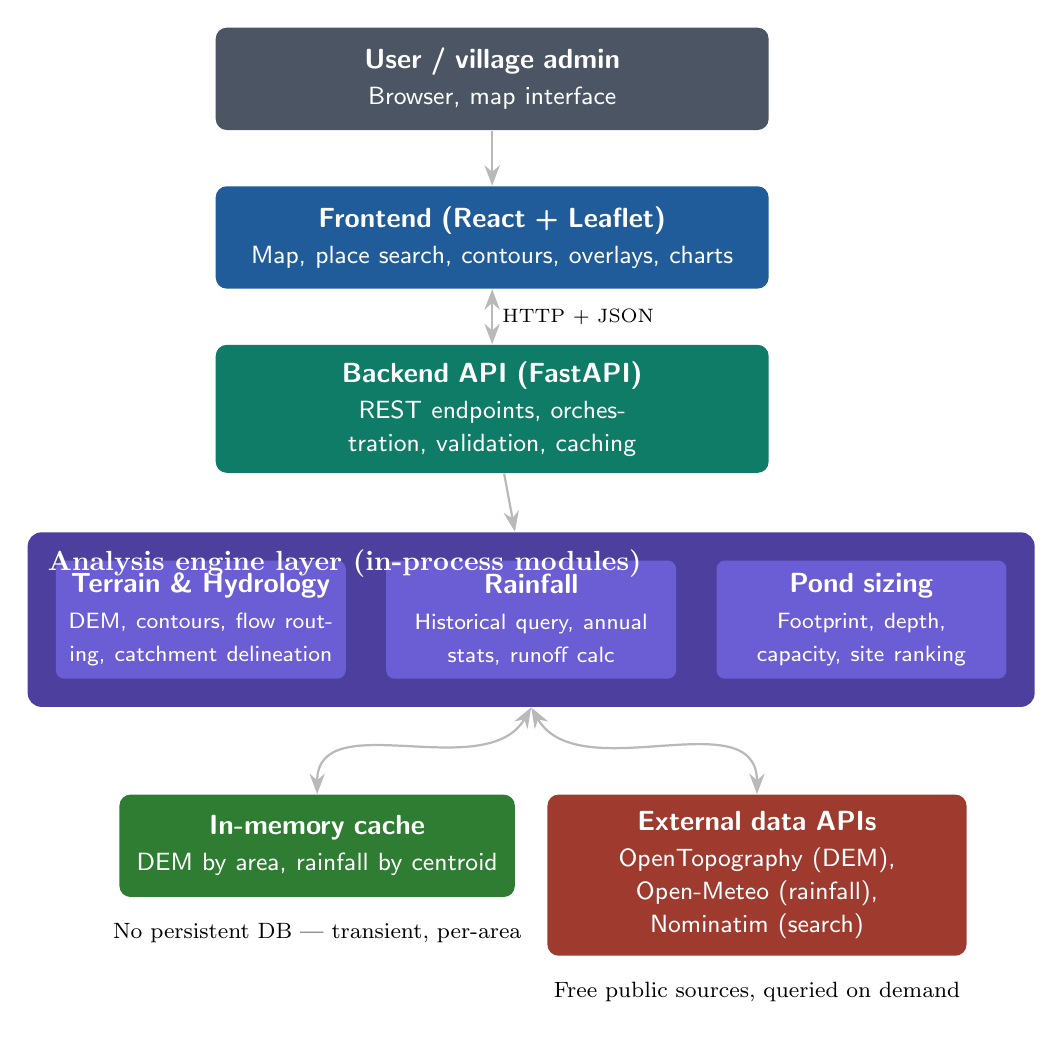
\begin{tikzpicture}[
    font=\sffamily,
    lay/.style={rounded corners=4pt, align=center, inner sep=6pt, text=white, minimum height=13mm},
    sub/.style={rounded corners=3pt, align=center, inner sep=4pt, text=white, fill=cSub, text width=3.4cm, minimum height=15mm},
    note/.style={align=center, font=\footnotesize, text=black},
    arr/.style={-{Stealth[length=2.6mm]}, thick, gray!55},
    darr/.style={{Stealth[length=2.6mm]}-{Stealth[length=2.6mm]}, thick, gray!55},
  ]
  % --- vertical spine ---
  \node[lay, fill=cUser, text width=6.6cm] (user) {\textbf{User / village admin}\\[1pt]\small Browser, map interface};
  \node[lay, fill=cFront, text width=6.6cm, below=7mm of user] (fe)
    {\textbf{Frontend (React + Leaflet)}\\[1pt]\small Map, place search, contours, overlays, charts};
  \node[lay, fill=cBack, text width=6.6cm, below=7mm of fe] (be)
    {\textbf{Backend API (FastAPI)}\\[1pt]\small REST endpoints, orchestration, validation, caching};

  % --- analysis engine layer: title + three sub-modules ---
  \node[below=9mm of be] (aeltitle) {};
  \node[sub, anchor=north] (terrain) at ([xshift=-3.7cm,yshift=-2mm]aeltitle.north)
    {\textbf{Terrain \& Hydrology}\\[1pt]\footnotesize DEM, contours, flow routing, catchment delineation};
  \node[sub, right=5mm of terrain] (rain)
    {\textbf{Rainfall}\\[1pt]\footnotesize Historical query, annual stats, runoff calc};
  \node[sub, right=5mm of rain] (pond)
    {\textbf{Pond sizing}\\[1pt]\footnotesize Footprint, depth, capacity, site ranking};
  \begin{scope}[on background layer]
    \node[fit=(terrain)(rain)(pond), rounded corners=5pt, fill=cAnalysis, inner sep=10pt] (ael) {};
  \end{scope}
  \node[anchor=north west, text=white, font=\bfseries] at ([shift={(4pt,-3pt)}]ael.north west)
    {Analysis engine layer (in-process modules)};

  % --- bottom layer: cache + external APIs ---
  \node[lay, fill=cCache, text width=4.6cm, below left=11mm and 0.2cm of ael.south]
    (cache) {\textbf{In-memory cache}\\[1pt]\small DEM by area, rainfall by centroid};
  \node[lay, fill=cExt, text width=4.9cm, below right=11mm and 0.2cm of ael.south]
    (ext) {\textbf{External data APIs}\\[1pt]\small OpenTopography (DEM), Open-Meteo (rainfall), Nominatim (search)};

  \node[note, below=2mm of cache] {No persistent DB --- transient, per-area};
  \node[note, below=2mm of ext] {Free public sources, queried on demand};

  % --- arrows ---
  \draw[arr] (user) -- (fe);
  \draw[darr] (fe) -- node[right,font=\scriptsize,text=black]{HTTP + JSON} (be);
  \draw[arr] (be) -- (ael);
  \draw[darr] (ael.south) to[out=-120,in=90] (cache.north);
  \draw[darr] (ael.south) to[out=-60,in=90] (ext.north);
  \end{tikzpicture}}
  \caption{High-level system architecture. The user's browser talks to the React
  front-end, which calls the FastAPI backend; the backend orchestrates the
  in-process analysis engine (terrain/hydrology, rainfall and pond-sizing modules),
  an in-memory cache and the external data APIs. There is no persistent database.}
  \label{fig:architecture}
  \Description{A layered block diagram: user/browser at the top, then the React
  front-end, then the FastAPI backend, then an analysis engine layer containing
  terrain-and-hydrology, rainfall and pond-sizing modules, with an in-memory cache
  and external data APIs (OpenTopography, Open-Meteo, Nominatim) at the bottom.}
\end{figure}

\subsection{What happens on one request}
It is easiest to understand the design by following a single request end to end.
When the user frames an area and presses \emph{Analyse}, the front-end turns the
map selection into a bounding box and sends it as JSON to \texttt{POST
/analyzeArea}. The backend first validates the box (rejecting anything malformed,
too large or too small), then checks its in-memory cache. On a miss it asks
OpenTopography for a DEM covering exactly that box, requesting the plain-text ASCII
grid format so no heavyweight geospatial libraries are needed to read it. That
download is the slow part, so it is done asynchronously; the rest of the pipeline,
which is pure NumPy, then runs quickly on the result.

From the raster the backend builds an elevation grid and a slope map, fills small
artificial pits, computes flow direction and flow accumulation, and from the
accumulation marks the existing stream network. It scores every cell for pond
suitability, removes the steep cells and the stream cells, and picks a few
well-separated candidate sites. For each candidate it traces the catchment
upstream, works out the pond's own flooded footprint, measures both in metres, and
combines the catchment with the rainfall figure to estimate runoff, storage
capacity, the collectable volume and a depth--volume curve. It also generates
contour lines for display. Finally it packs everything --- candidates, contours,
drainage network, rainfall, a summary and a processing log --- into one JSON
response, which the front-end draws as layered overlays on the map. If any external
call fails, the request does not: rainfall falls back to a documented default, and
an unreachable DEM service returns a clear, actionable error instead of a stack
trace.

In short, the pipeline runs as: validate the box and check the cache; fetch the DEM
(async); build the elevation grid and slope; fill depressions, then D8 flow
direction, then flow accumulation; rank candidate sites (excluding steep ground and
channels); per site, trace the catchment and footprint and measure them in UTM;
query rainfall and compute runoff, capacity and the storage curve; and finally
assemble the JSON (with contours and the drainage network) that the front-end draws.

\subsection{Component responsibilities}
I kept each analysis module to a single, non-overlapping job so that a change in
one place does not ripple into another. \texttt{elevation\_api} fetches and parses
the DEM; \texttt{terrain\_grid} builds the grid and slope; \texttt{catchment} does
the depression filling, flow direction, flow accumulation and watershed tracing;
\texttt{pond\_locator} scores and ranks the sites; \texttt{geometry\_utils}
measures areas and perimeters in metres; \texttt{rainfall\_api} handles rainfall;
\texttt{water\_volume} does the runoff, capacity and storage-curve maths;
\texttt{contour\_lines} produces the contours for display; and
\texttt{visualization} renders the downloadable figure. The route handler itself
stays thin and just calls these in order. On the front-end the split is similar:
\texttt{App} holds the state and controls, \texttt{MapView} owns the Leaflet map and
all the overlays, \texttt{ResultsPanel} shows the per-site numbers and charts, and
\texttt{Search} does the place lookup.

\subsection{Deployment view}
On each server the built front-end is copied into the backend and served from
there, and the process is started detached (with \texttt{nohup}) so it survives the
session ending. Inside the container it listens on port 5000, which is forwarded
out to port 5228, so the app is reached at the external address. Dependencies are
installed into the environment already present on the machine rather than a fresh
virtual environment, which keeps the storage footprint down. Because the whole
system is one dependency-light process, the identical build runs on any of the four
provided machines without modification.

\subsection{Technology Stack}
On the backend I used Python with FastAPI, which gives an async web layer and
auto-generated API docs for free. NumPy and SciPy do the raster and hydrology work;
Shapely and pyproj handle the polygon geometry and the UTM projection; contourpy
extracts the contour lines; httpx makes the async external calls; and matplotlib
(imported only when a figure is actually requested) renders the downloadable image.
The front-end is React, bundled with Vite, using Leaflet for the map, with
OpenStreetMap as the base layer and Esri World Imagery available as a satellite
toggle. For data, elevation comes from the OpenTopography Global DEM API (SRTMGL1,
30\,m), rainfall from the Open-Meteo historical archive, and place search from
OpenStreetMap's Nominatim service.

Some of this differs from the stack suggested in the brief, and those changes were
deliberate. The brief pointed at per-point elevation services and a PostGIS
database. I moved to OpenTopography because it returns a whole DEM raster for the
selected area in one request; the per-coordinate services I tried first kept
hitting rate limits and became unusable during development. And I dropped the
database entirely, because the analysis holds no state worth persisting and the
containers are too storage-limited to justify one (Section~\ref{sec:db}). The
satellite-based existing-pond detection sketched in the high-level design was left
out of this phase.

%% =====================================================================
\section{Methodology}
\label{sec:methodology}
This section explains the actual algorithms behind the pipeline.

\subsection{Terrain and Elevation Analysis}
For the chosen bounding box the backend requests a DEM from OpenTopography
(SRTMGL1, 30\,m) in ESRI ASCII-grid form, which is plain text and can be read with
NumPy alone --- no native GDAL or rasterio build is needed, which matters on the
lab containers. I orient the raster so that latitude increases with the row index,
fill in any no-data cells, and, if the grid is larger than a set cap, downsample it
by a fixed stride to keep memory in check. Slope at each cell comes from the Horn
(1981) finite-difference gradient,
$\text{Slope}=\arctan\!\sqrt{(dz/dx)^2+(dz/dy)^2}$, after converting the cell
spacing from degrees to metres. The elevation contours shown on the map are pulled
straight from this grid using contourpy.

\subsection{Catchment Area Delineation}
A coarse DEM has small spurious pits that would trap water, so I first fill them
with the Priority-Flood algorithm (Barnes et al., 2014), an $O(n\log n)$ method
that processes cells outward from the boundary in order of elevation. Next, D8 flow
direction (O'Callaghan \& Mark, 1984) sends each cell to its steepest downhill
neighbour, and flow accumulation --- how many upstream cells drain through each one
--- is found by walking the flow graph in topological order. To get the catchment
of a candidate site I trace this graph backwards from the site, adding a neighbour
whenever its flow direction points at the current cell, until nothing upstream is
left. The resulting set of cells is unioned into an exact polygon (I avoided a
convex hull here, since testing showed it inflated the area badly) and reprojected
into the local UTM zone, chosen automatically from the location, so the area and
perimeter come out in metres. Two assumptions are worth stating: D8 sends all of a
cell's flow to one neighbour, and at 30\,m the small valley-scale drainage on flat
ground is only roughly captured, so catchments in flat areas are on the
conservative side.

\subsection{Rainfall Data Integration}
Mean annual rainfall for the centre of the area comes from the Open-Meteo
historical archive, using the daily precipitation totals and averaging over the
last several complete years so that one unusually wet or dry year does not skew the
figure; a month-by-month climatology is returned as well for the chart. Every call
has a timeout, and if the archive cannot be reached the system falls back to a
documented default annual rainfall and labels the source as such, so a volume
estimate is always available.

\subsection{Pond Siting and Water Volume}
Two terrain measures decide where a pond makes sense. The Topographic Wetness Index,
$\text{TWI}=\ln(a/\tan\beta)$, captures how strongly water gathers at a cell given
its slope, and the Topographic Position Index,
$\text{TPI}=z-\overline{z}_{\text{nbhd}}$, captures whether a cell sits below its
surroundings. I combine them as $\text{Score}=0.5\,\text{TWI}_n +
0.5\,(-\text{TPI})_n$, then exclude anything steeper than $15^\circ$, any cell in
the existing channel network (flow accumulation above the 97th percentile plus a
buffer), and any candidate whose flooded footprint cannot be contained. For volume,
the runoff the catchment delivers in a year is estimated with the Rational method,
$V_{\text{runoff}}=C\,P\,A_{\text{catchment}}$ with $C=0.3$ by default; the basin's
storage capacity is read straight off the DEM as $\sum(w-z_i)A_{\text{cell}}$; and
the water that can actually be collected is the smaller of the two,
$\min(V_{\text{runoff}},V_{\text{capacity}})$. I also build a stage--area--volume
curve and report the depth at which the stored volume first reaches a year's runoff.
The suitability score is what \emph{finds} the candidate sites, but the list the user
sees is then ordered best-first by this collectable volume, so Rank~1 is the site
that actually harvests the most water rather than just the highest-scoring terrain.

%% =====================================================================
\section{Implementation}
\label{sec:implementation}

\subsection{Backend and API Design}
The backend exposes a small REST surface (Table~\ref{tab:api}). Everything goes in
and out as JSON, the shapes are defined with Pydantic models, and FastAPI turns
those into interactive documentation at \texttt{/docs} on its own. There is no
authentication --- it is an open, read-only analysis tool for the demo. Failures
from the third-party APIs are handled explicitly rather than left to bubble up: a
bad or out-of-range area gives back \texttt{422}, an unreachable elevation service
gives \texttt{502} with a message the user can act on, a rainfall failure quietly
uses the fallback, and any unexpected error in a stage returns \texttt{500} naming
the stage that broke.

\begin{table}[h]
  \caption{REST API endpoints}
  \label{tab:api}
  \begin{tabular}{p{4.0cm}p{3.5cm}}
    \toprule
    Method \& path & Purpose \\
    \midrule
    \texttt{POST /analyzeArea} & Analyse a selected map region (bbox) \\
    \texttt{POST /analyzeArea?format=image} & Same, returns a rendered PNG \\
    \texttt{POST /analyzeContour} & Analyse an uploaded contour KML/KMZ (Phase 2) \\
    \texttt{GET /health} & Service health check \\
    \texttt{GET /docs} & Auto-generated API documentation \\
    \bottomrule
  \end{tabular}
\end{table}

\subsection{Frontend and Visualization}
The front-end (Figure~\ref{fig:ui}) is a single-page React and Leaflet app. The
user can type a village or town name to jump the map there, frame a village-sized
block, and select it either with a one-click ``use current view'' button or by
clicking two opposite corners of a rectangle --- I added the two-click option
because click-and-drag was awkward on a laptop trackpad. Once the analysis returns,
the map layers on the elevation contours, the existing drainage in blue, and for
each ranked site the pond footprint as a filled shape labelled with its area, the
catchment as a dashed outline, and a marker at the pond point. The side panel lists
the catchment area, pond footprint, annual runoff, basin capacity, collectable
volume and required depth for each site, with a small storage-curve chart and a
monthly rainfall chart, and the results can be downloaded as a PNG, as GeoJSON or
as the full JSON.

\begin{figure}[h]
  \centering
  \IfFileExists{figures/ui.png}
    {\includegraphics[width=\linewidth]{figures/ui.png}}
    {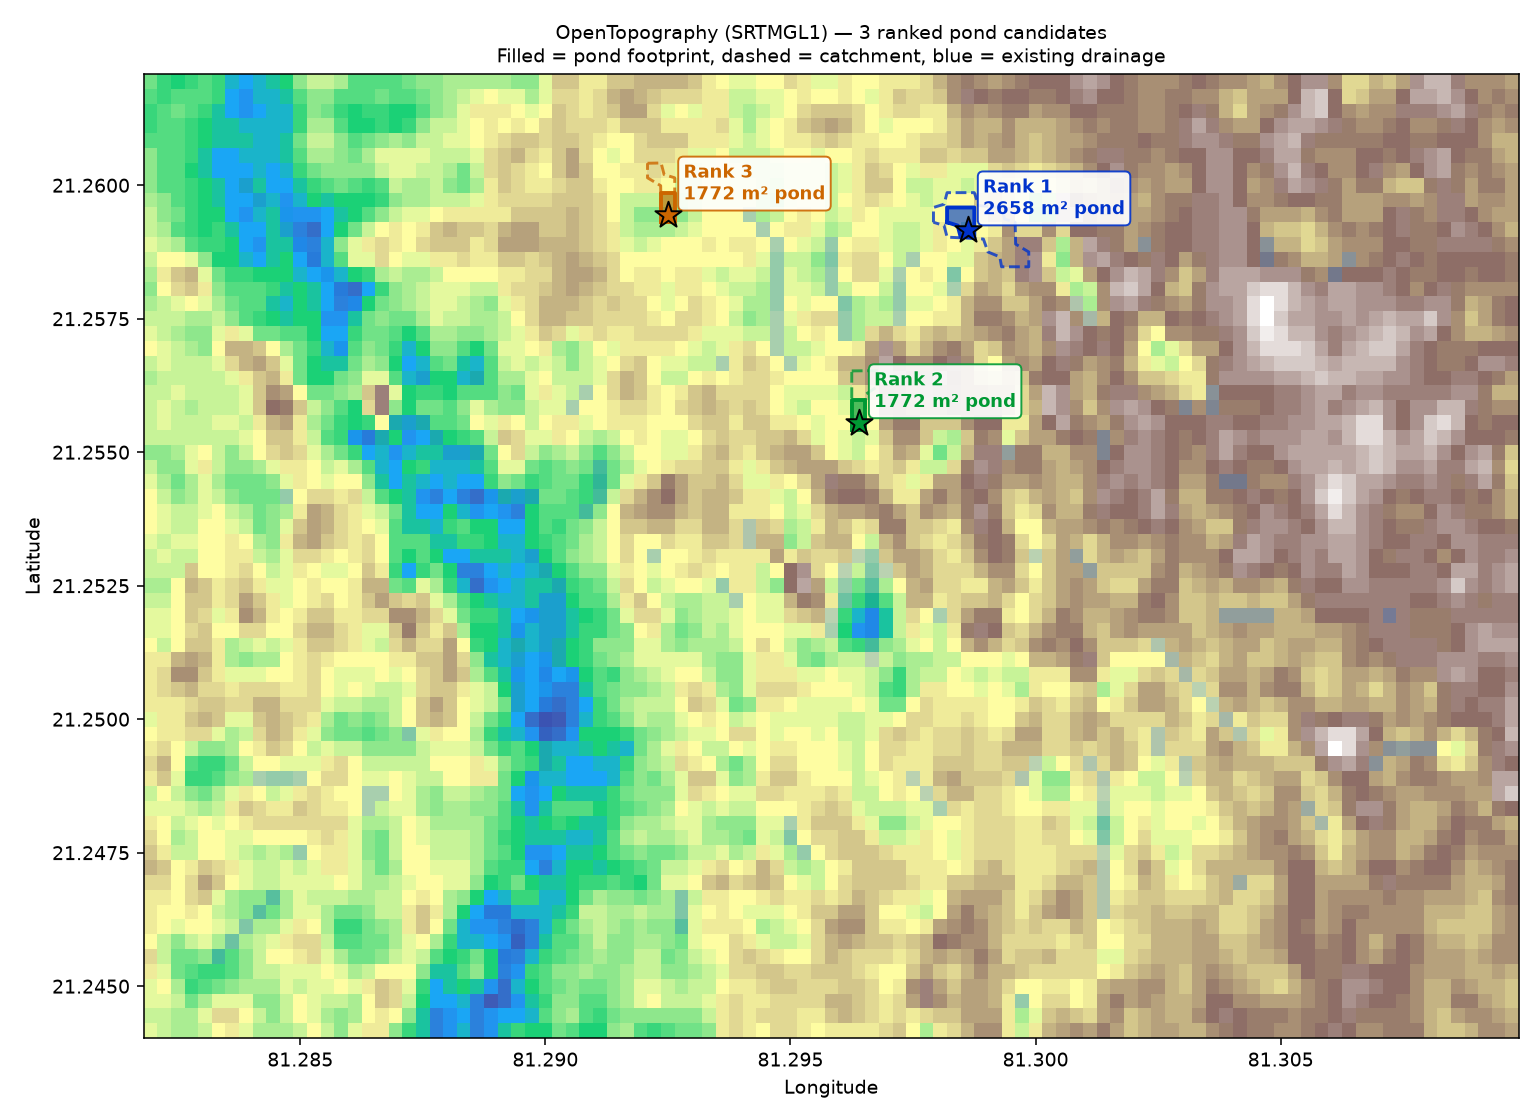
\includegraphics[width=\linewidth]{figures/sample_analysis.png}}
  \caption{Application results for the sample region: DEM terrain shading, the
  existing drainage network (blue), and three ranked pond sites (filled
  footprints) with their catchments (dashed), all kept off the watercourses.}
  \label{fig:ui}
  \Description{A rendered map of the sample area showing terrain, blue drainage
  channels, and three suggested ponds placed away from the drainage with their
  catchment outlines.}
\end{figure}

\subsection{Database and Storage}
\label{sec:db}
There is no persistent database. Each analysis is computed on the spot from live
data and returned; there is simply no cross-session state to keep. To avoid asking
the external APIs for the same thing twice, the fetched DEMs (keyed by bounding
box) and rainfall results (keyed by the centre point) are held in an in-memory
cache, which is why re-analysing the same or a nearby area comes back instantly.
This was a conscious choice: the containers are tight on storage and memory, a
database would add weight and one more thing that can fail for no real benefit
here, and staying stateless is what lets the same build run on any of the four
machines without setup. If the user wants to keep a result, the GeoJSON and JSON
downloads let them do that locally.

%% =====================================================================
\section{CSD Themes and Topics Applied in the Project}
\label{sec:csd-themes}
Table~\ref{tab:csd-themes} connects the course's system-design themes to where each
one actually shows up in this project. Where I did not implement a theme, I have
said so plainly and given the reason, rather than claim it.

\begin{table*}[t]
  \caption{Mapping of core CSD themes/topics to their use in this project}
  \label{tab:csd-themes}
  \begin{tabular}{p{2.8cm}p{5.2cm}p{6.5cm}}
    \toprule
    CSD Theme/Topic & Where used in the project & Justification / design rationale \\
    \midrule
    API Design (REST) & \texttt{POST /analyzeArea}, \texttt{/analyzeContour}, \texttt{/health} & A clear JSON request/response contract via Pydantic, with docs generated automatically; a query flag (\texttt{format=image}) switches the representation without needing a separate route. \\
    Caching & In-memory cache of DEM (by bbox) and rainfall (by centroid) & The external DEM download dominates the response time; caching turns repeat and nearby analyses into instant responses and removes duplicate external calls. \\
    Concurrency / Asynchronous Processing & \texttt{async} route with \texttt{httpx.AsyncClient} for the DEM fetch & The request is I/O-bound on the external API, so an async fetch keeps the event loop free; the fast NumPy pipeline runs once the data is back. \\
    Monolith vs. Microservices & One FastAPI process serving both the API and the static front-end & I chose a monolith over the microservice sketch in the HLD because the containers are tiny (512\,MB) and one process keeps memory, deployment steps and failure points to a minimum. \\
    Error Handling and Resilience & Rainfall fallback, DEM 502 with guidance, bbox validation, retry/backoff & The system depends on free external APIs, so it has to degrade gracefully instead of failing a whole analysis; every failure has a defined behaviour. \\
    Algorithms and Complexity & Priority-Flood ($O(n\log n)$), D8 + flow accumulation ($O(n)$), BFS watershed & Using optimal/linear algorithms keeps the compute negligible ($\sim$0.1\,s), so the total time is set by the network, not the CPU. \\
    Geospatial / Projection & UTM projection (pyproj), exact cell-union polygons (Shapely) & Areas have to be measured in metres, not degrees; the exact union avoids the roughly 78\% overestimate a convex hull gave in testing. \\
    Resource-Constrained Design & Lazy matplotlib import, grid cap + downsampling, point caps & These keep the resident memory around 160\,MB, comfortably under the 512\,MB container limit. \\
    Testing Strategy & 71 unit and integration tests (Section~\ref{sec:results}) & Each module is tested on its own plus end to end, which gives confidence the pipeline is right and that refactoring it is safe. \\
    Containerization / Deployment & Runs in the provided Docker containers; scripted pull + restart on internal port 5000 (forwarded to 5228) & Reproducible and redeployed with one command; it uses the environment already on the machine instead of a duplicate virtual environment to save space. \\
    Version Control & Git and GitHub, small incremental commits & The history records every change and fix and keeps the deployed servers in sync through \texttt{git pull}. \\
    Load Balancing & Not implemented & A single instance handles the expected demo load within the container; an Nginx reverse proxy across instances would be the way to scale out. \\
    Authentication / Authorization & Not implemented & The tool is an open, read-only analysis service for the demo and stores no user data. \\
    Database Indexing & Not applicable & There is no persistent database (Section~\ref{sec:db}); state is transient and cached in memory. \\
    CI/CD & Not implemented & Deployment is a scripted \texttt{git pull} and restart, and the tests are run by hand before deploying. \\
    \bottomrule
  \end{tabular}
\end{table*}

If I had to point to the three decisions that mattered most, they would be caching,
resilience and the choice of a monolith. Caching mattered because a single analysis
is dominated by the roughly twelve-second DEM download; keying the cache on the
bounding box turns any repeat or nearby selection into an instant response, which is
what actually makes exploring the map usable. Resilience was not really optional:
early on, the free per-coordinate elevation service kept hitting rate limits and the
other providers I tried were unreachable, so I moved to OpenTopography's
single-request raster and made every external call fail softly --- rainfall drops to
a default, and elevation returns a message the user can act on. And I went with a
monolith instead of the microservice design in the original plan precisely because
the targets are 512\,MB containers; one small process that serves both the API and
the web app is the design that fits the hardware I was given.

%% =====================================================================
\section{Results and Evaluation}
\label{sec:results}
Figure~\ref{fig:ui} shows the system run on the sample region we were provided (near
Raipur, Chhattisgarh). The 30\,m DEM (elevations of 266--298\,m) reproduces the
landscape you would expect: the diagonal blue band is the main stream valley with
its tributaries, and all three suggested ponds land on drainable ground clear of
that network. Table~\ref{tab:results} gives the numbers.

\begin{table}[h]
  \caption{Ranked pond candidates for the sample region ($C=0.3$).
  Catchment area is always $\geq$ pond footprint, as expected.}
  \label{tab:results}
  \small
  \begin{tabular}{clrrrr}
    \toprule
    Rank & Location (lat, lon) & Catch. & Pond & Collect. & Depth \\
         &                     & (m$^2$)& (m$^2$)& (m$^3$/yr) & (m) \\
    \midrule
    1 & 21.2592, 81.2986 & 6\,202 & 2\,658 & 1\,901 & 2.5 \\
    2 & 21.2556, 81.2964 & 2\,658 & 1\,772 & 877   & 1.0 \\
    3 & 21.2594, 81.2925 & 2\,658 & 1\,772 & 877   & 1.0 \\
    \bottomrule
  \end{tabular}
\end{table}

The numbers hang together the way they should: the catchment (the source of the
water) is always at least as big as the pond footprint (where the water sits), and
the collectable volume is the smaller of what the catchment can deliver and what
the basin can hold. As a sanity check I compared this against Phase 2, which used a
1\,m contour map of the same area, and the pipeline picks the same drainable zones
and keeps clear of the river.

\subsection{Performance}
A fresh analysis of a new area takes about twelve seconds, and almost all of that
--- around 11.6\,s --- is the OpenTopography download; the entire CPU pipeline (flow
routing, siting, catchment, geometry and volume) runs in roughly 0.1 to 1.5\,s. Once
an area is cached the response comes back in well under a second. The server sits at
about 160\,MB of resident memory, well below the 512\,MB limit. The backend passes
71 automated tests covering the parser, terrain grid, flow and catchment, pond
locator, geometry, elevation parsing, rainfall, water volume and the image-rendering
path.

%% =====================================================================
\section{Discussion and Limitations}
\label{sec:discussion}
On the whole the pipeline works reliably and I can explain every step of it, and
moving to OpenTopography's single-request raster was what turned a flaky prototype
into something dependable after the per-coordinate services had let me down. The
real limits come from the free data and the scope I set. At 30\,m the DEM cannot
resolve small valley-scale drainage on flat ground, so catchments there stay modest
and the D8 watershed can break into pieces; areas with genuine relief give much
larger and cleaner catchments. The rainfall archive is sometimes unreachable, and
when it is the system uses a documented fallback value and flags it, which makes
those particular volume figures indicative rather than exact. The system also
reasons only from terrain and rainfall: it does not know whether water already sits
at a spot, and it does not do the civil design of the pond. None of
these are bugs --- they follow from the input data and the scope --- but they are
the reason the output is best treated as a shortlist to check on the ground rather
than a final design.

%% =====================================================================
\section{AI Tool Usage Declaration}
\label{sec:ai-usage}
I used Claude while working on this project. It helped me draft first versions of
some of the modules, talk through the terrain-analysis algorithms I was
implementing, and track down a few bugs during testing --- for example, a case where
a pond's footprint came out larger than its own catchment, which I fixed by clipping
the footprint to the catchment, and the elevation service hitting rate limits, which
led me to switch providers and add fallbacks. It also helped me fit this write-up
into the report template. I went through everything it produced, changed what needed
changing, and I can explain the algorithms and the design decisions in this report
on my own.

%% =====================================================================
\appendix

\section{Source Code and Repository}
The full source code, the commit history and this report live at
\url{https://github.com/krish1809/village-pond}, and the running application is at
\url{http://10.1.75.79:5228/} (with the API docs at \texttt{/docs}). The repository
is laid out as follows: \texttt{backend/} holds the FastAPI service, with
\texttt{modules/} for the analysis code, \texttt{api/routes/} for the endpoints,
\texttt{models/} for the Pydantic schemas and \texttt{tests/} for the tests;
\texttt{frontend/} holds the React and Leaflet app under \texttt{src/};
\texttt{scripts/} holds the build and deploy scripts; \texttt{docs/} holds the
design documents and this report; and the sample contour file sits at the project
root.

\end{document}
\endinput
